%%%%%%%%%%%%%%%%%%%%%%%%%%%%%%%%%%%%%%%%%%%%%%%%%%%%%%
%\section{Human Activity Recognition}
%%%%%%%%%%%%%%%%%%%%%%%%%%%%%%%%%%%%%%%%%%%%%%%%%%%%%%
\label{sec:HAR}

In this section we describe the implementation of the human acitivity
recognition ('HAR') component on the mobile device.  The algorithmic
foundation of this data mining task have been described in detail in
deliverable D2.2 in section 3.2 ``Mobile Sensing and activity
recognition''. We include a brief summary here (\ref{sec:har_method})
for the sake of completeness. Subsection \ref{sec:har_component}
contains the descriptions of the implementation. In subsection
\ref{sec:har_eval} we evaluate our method to the on two data sets and
compare it to the state of the art approaches.

\subsection{HAR Method Summary}\label{sec:har_method}

The process of activity recognition uses a pipeline of signal
processing and machine learning techniques. It consists of two phases:
the ``training phase'' and the ``integration phase''. 

\begin{figure}[htbp]
\centering
\subfigure[HAR Training Phase]{
\label{fig:har_overview}
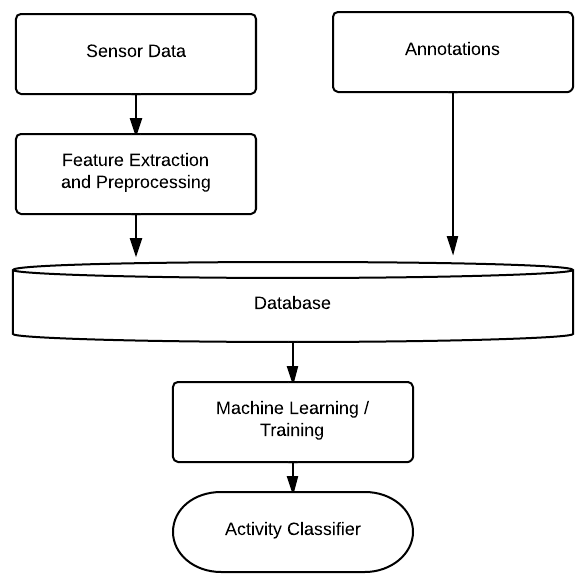
\includegraphics[width=0.5 \textwidth]{img/har/classification_overview.png}
}
\subfigure[HAR Integration Phase]{
\label{fig:integrated_har_overview}
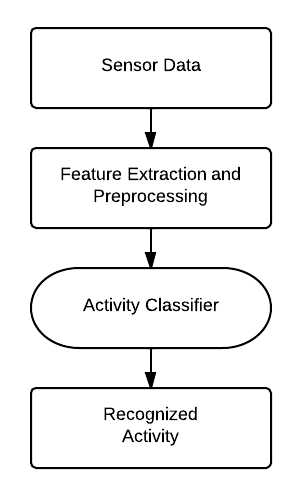
\includegraphics[width=0.25 \textwidth]{img/har/integration_overview.png}
}
\caption{Overview Human Activity Recognition}
\end{figure}


In the training phase (cf. Figure \ref{fig:har_overview}) a group of
volunteers is asked to perform the targeted activities for a certain
amount of time, while recording sensor samples with the device in
their pocket.  The gained training data stored in a database and used
to train a classifier of the activities.

In the integration phase (cf. \ref{fig:integrated_har_overview}), the
trained classifier is embedded into the mobile device.

Both phases rely on the preprocessing steps of "windowing'' and
``feature generation''. The stream of incoming sensor data is divided into
time windows of fixed size (typically 1-10 sec.) and for each window
a set of features is computed. This features are filtering out
relevant information from the raw signal. Typical features include
mean values and standard deviations as well as frequency domain
features like Fourier modes.

Deliverable D2.2 contains detailed lists of all sensors and features
and data mining methods that are used in the literature as well as
discussions of quality of the recognition results.

\subsection{Component Description}\label{sec:har_component}

Architecture Description.

\begin{figure}[htbp]
\centering
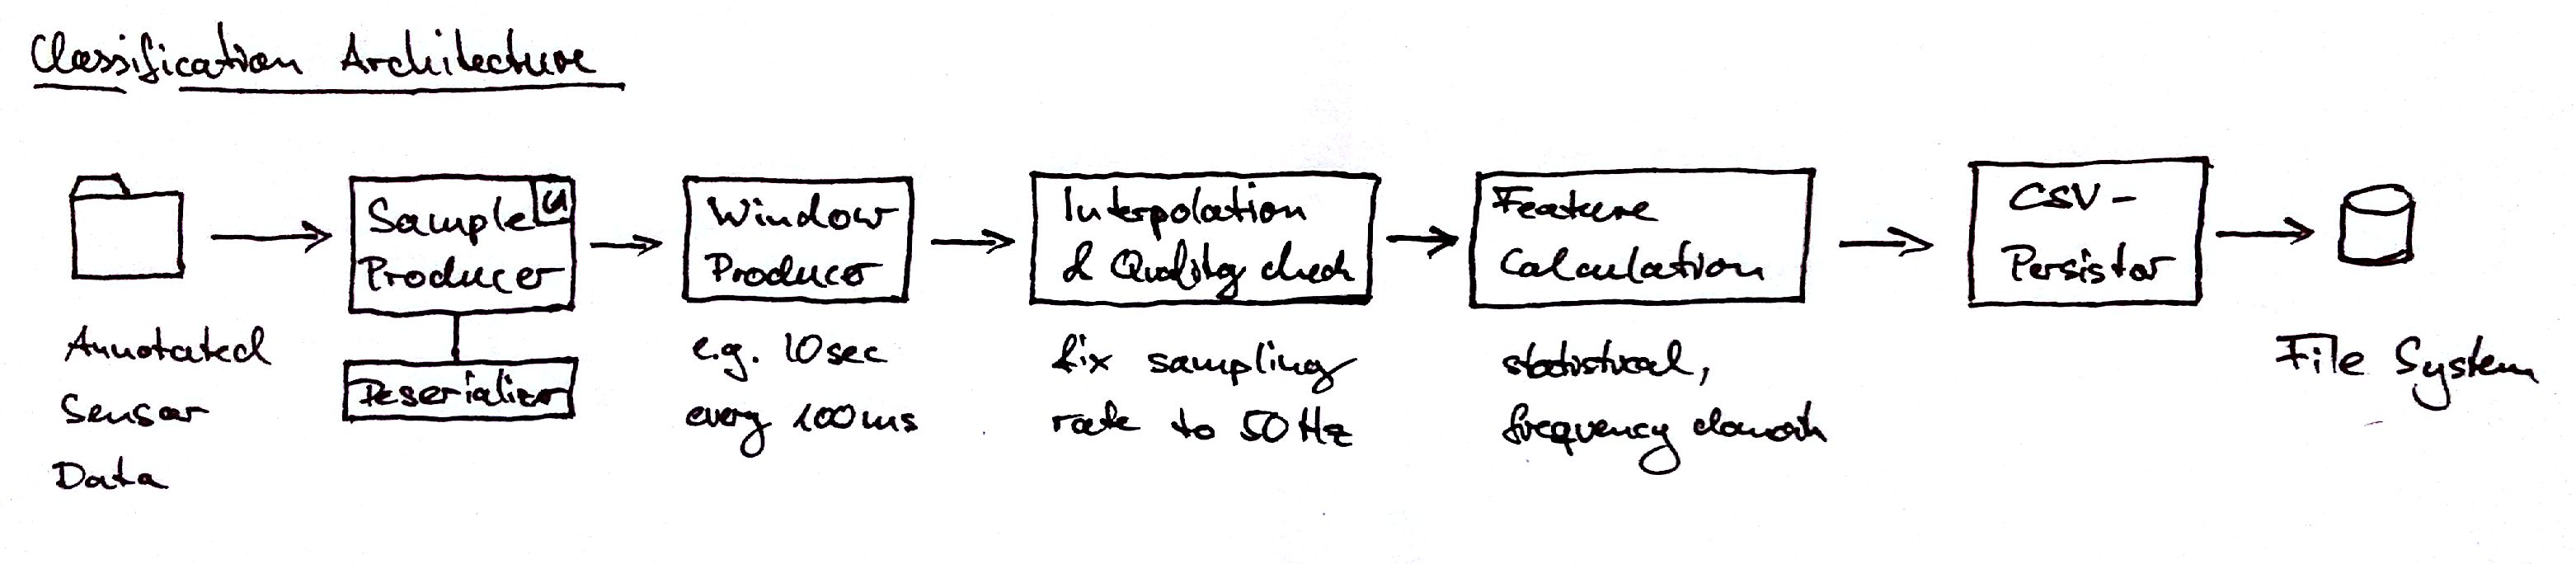
\includegraphics[width=\textwidth]{img/har/classification_architecture.jpg}
\caption{Classification Architecture}\label{fig:classification_architecture}
\end{figure}

\begin{figure}[htbp]
\centering
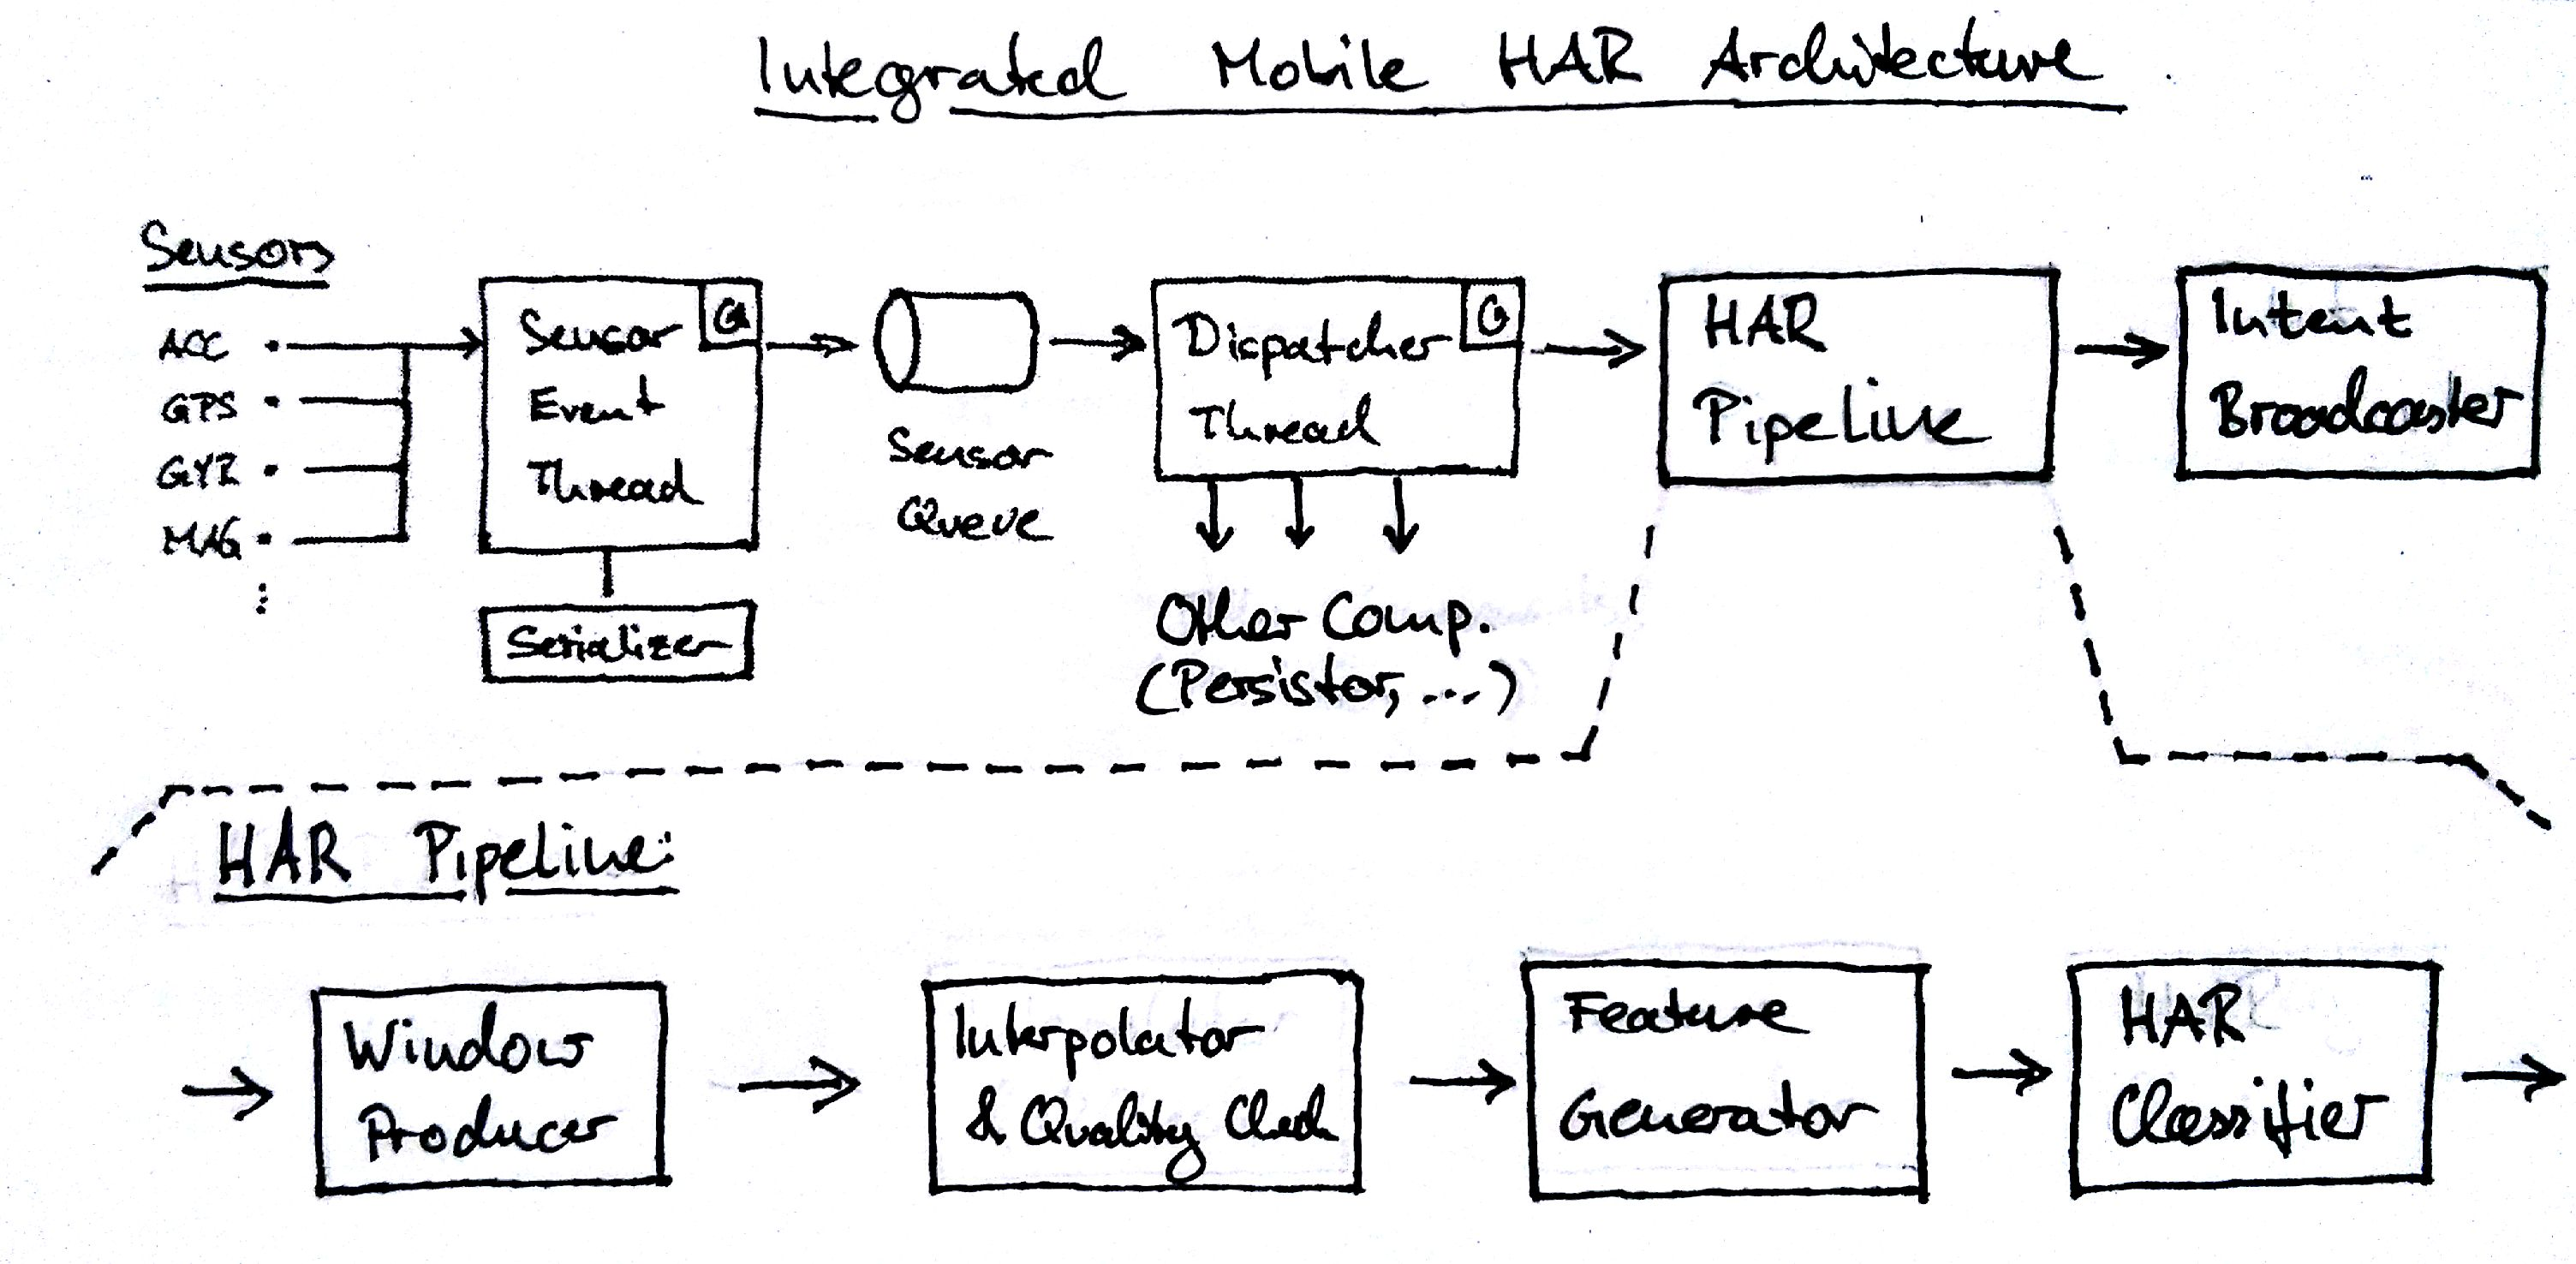
\includegraphics[width=\textwidth]{img/har/integration.jpg}
\caption{Integrated HAR Architecture}\label{fig:integrated_har}
\end{figure}

% TODO CE
% Describe the component implementation.
% This can be done in a similar fashion like the sensor collector
% further up: Add Bullet point list for the individual components.
% And describe them in one or two sentences.
% * Add a list for the features we use in the current implementation
% * Describe how we train the decision tree classifier using WEKA.
%   Add a screenshot of the results. 
% * Describe how we integrate the classifier into the application

% TODO:
% * Describe Dection Tree Classifier [HH]
% * Describe SVM [CERTH]

\subsection{Evaluation}\label{sec:har_eval}

We have evaluated our classifier on two different datasets.

The first dataset was gathered on the University Campus in Koblenz in
December 2013.  It contains a total of around $900K$ samples collected
by $10$ volunteers.  The volunteers were instructed to perform the
activities ''walking'', ''running'', ''stairs'' and ''cycling'' on
predefined routes on the university campus (cf. Figure
\ref{fig:data_collection_handout}). The total time effort per
volunteer was about 20-25minutes and a financial reward was offered as
an incentive. After the recording the samples have been inspected
using our inspection tool and the beginning and ending of the
activities were manually stripped in order to avoid noise from holding
the device in the hand.

%
% [TODO: Publication of Dataset!]
%

The other dataset was obtained from the {\it UCI Machine Learning
  Repository}\footnote{\url{http://archive.ics.uci.edu/ml/datasets/Human+Activity+Recognition+Using+Smartphones}}
and was gathered by Davide Anguita, et. al. \cite{Anguita} in 2012.
It contains around $700K$ collected by 30 volunteers.

The number of samples per activity of both datasets are summarized in
Figure \ref{fig:har_datasets}. Both datasets contain only
accelerometer samples, and have been preprocessed that have been
sampled at a fixed rate of $50Hz$.

\begin{figure}
\centering
\begin{tabular}{|l|r|r|} \hline
Activity  & UCI Dataset & UKOB Dataset \\ \hline
sitting   & 113.728     & 80.951        \\
standing  & 121.984     & 320.737       \\
walking   & 110.208     & 292.024       \\
running   & 0           & 31.916        \\
cycling   & 0           & 436.106       \\
stairs    & 188.800     & 30.086        \\
lying     & 124.416     & 0            \\ \hline \hline
Totals    & 659.136     & 903.156       \\ \hline
\end{tabular}

\caption{Number of accelerometer samples by activity and dataset.}
\label{fig:har_datasets}
\end{figure}

\begin{figure}[htbp]
  \centering
  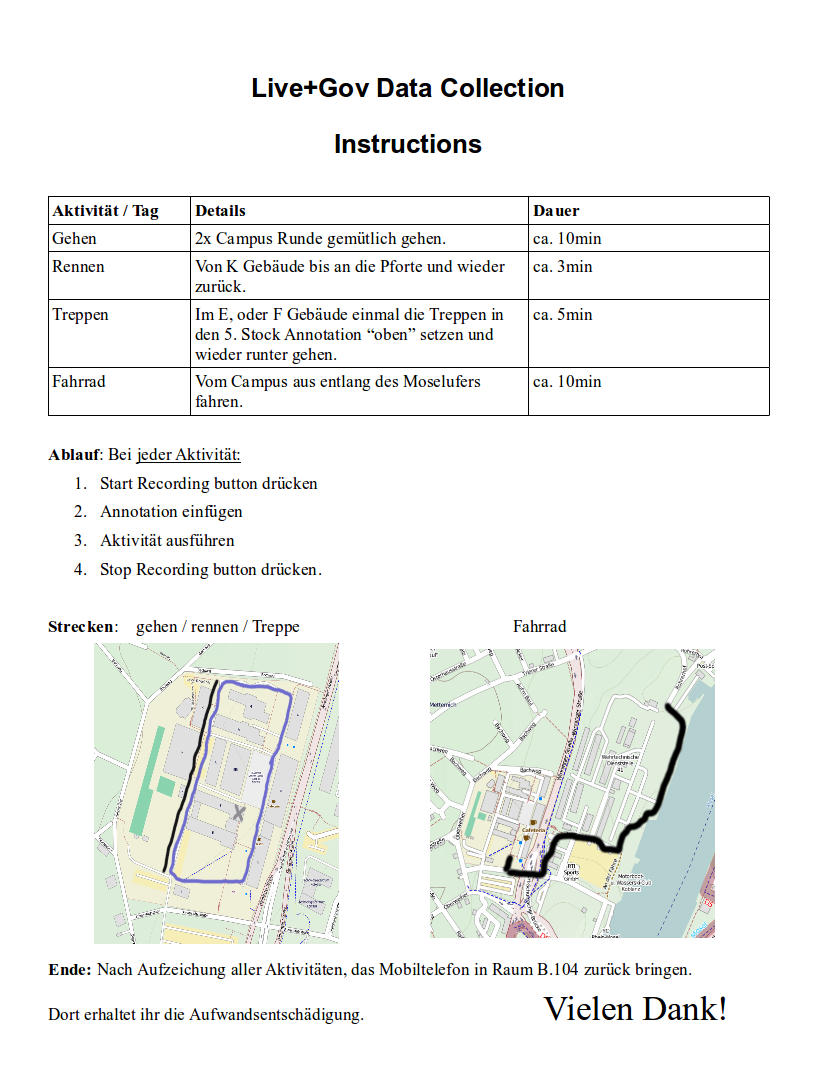
\includegraphics[width=\textwidth]{img/har/data_collection_handout.png}
  \caption{Instructions for data collection in German
    language}\label{fig:data_collection_handout}
\end{figure}


%
% TODO: Describe Evaluation Results
%


%%% Local Variables:
%%% mode: latex
%%% TeX-master: "../D1-2"
%%% End:
